%\documentclass[12pt, preprint,numberedappendix]{emulateapj}
%\documentclass[12pt, preprint]{aastex}
%\documentclass[apj]{emulateapj}
\documentclass[12pt, letterpaper]{article}

%\newcommand\submitms{n}		% set to y to follow AAS ``ms'' names, etc.
%\newcommand\bibinc{n}		% set to y if bib pasted in .tex, set to n to use bibtex


%\usepackage{pdfsync}
%\usepackage{subeqnarray}
\usepackage[top=0.9in, bottom=0.8in, left=1in, right=1in]{geometry}
\usepackage{natbib}
\usepackage{color}
\usepackage{graphicx}
\usepackage{fancyhdr}
\usepackage[T1]{fontenc}
\usepackage{titling}
\usepackage{sectsty}
\usepackage{sidecap}
\usepackage{placeins}
\usepackage{indentfirst}
\setlength{\droptitle}{-7em}
\setlength{\abovecaptionskip}{-0.4ex}
\setlength{\belowcaptionskip}{-0.4ex}
%\pagenumbering{gobble}
\pagestyle{fancy}
\lhead{Ana-Maria Piso}
\rhead{ITC Postdoctoral Fellowship Research Proposal}
\date{}
%\rhead{\thepage}


%\bibliographystyle{apj}

\title{ITC Postdoctoral Fellowship Research Proposal: \\
The Role of Disk Volatile Chemistry and Dynamics in Shaping the Compositions of Nascent Planets}
\author{Ana-Maria Piso}

%\newenvironment{packed_item}{
%\begin{itemize}
%  \setlength{\itemsep}{1pt}
%  \setlength{\parskip}{0pt}
%  \setlength{\parsep}{0pt}
%}{\end{itemize}}

\begin{document}
\maketitle

%\slugcomment{Draft Modified \today}

\vspace{-0.9cm}


Within the last two decades, more than one thousand extrasolar planets (exoplanets) have been discovered $[1]$. Their diversity in terms of mass, radius, location and composition $[2]$ provides an exciting field of research, with the eventual goal of finding planets that are similar to our own Earth and may sustain life. For this purpose, it is thus crucial to explore and understand how planets obtain their compositions. Observations of Earth-like planets that can provide useful insight about their composition are challenging --- the solid interior structure of terrestrial planets cannot be detected, and their gaseous envelopes are small by comparison (both in mass and radius), which makes it difficult to obtain atmospheric spectra and find out what chemical compounds they are made of. We therefore turn to giant planets, which have provided a rich and intriguing research area for decades. Gas giants contain most of their mass in their atmosphere, hence their chemical composition is determined by that of their envelopes. The last few years have seen a substantial increase in the number of giant planets with observed atmospheric spectra (e.g., $[3]$, $[4]$), which has enhanced our understanding of these planets' chemical structure, and has provided us with quantitative information about the abundances of various compounds in their envelopes besides hydrogen and helium. Finally, gas giants shape the architecture of planetary systems and affect the delivery of volatile compunds to terrestrial planets, which has direct consequences for the habitability of worlds similar to our own. Thus testing theories of planet formation against gas giant compositions will help constrain planet formation theories more generally.     

Both terrestrial and giant planets are born in protoplanetary disks, which implies that their \textbf{compositions are determined by and tightly linked to the structure and composition of the disk}. The chemical and dynamical evolution of disks, as well the formation of giant planets have both been previously investigated in isolation. However, the coupled chemo-dynamical disk evolution, planet compositions, and most importantly the disk-planet connection have not yet been considered in detail. As shown in my work on the minimum core mass of gas giants ($[5]$, $[6]$), planet formation depends sensitively on disk physics and chemistry. \textbf{I propose to develop a holistic chemo-dynamical framework to explore how disk dynamics and chemistry, as well as the dynamics of nascent planets and planetesimals, regulate the compositions of mature giant planets.} Such a model will enhance our understanding of planetary structures by enabling us to predict what kind of planet compositions result from planet formation in different parts of the disk. Furthermore, this work provides essential context for characterizing the gas giants that instruments such as the James Webb Space Telescope (JWST) and the Transiting Exoplanet Survey Satellite (TESS) will one day discover. 

\vspace{0.2in}

%\section{Coupled Chemical and Dynamical Disk Evolution} 
\underline{\textbf{1. Coupled Chemical and Dynamical Disk Evolution}}

Chemical and dynamical processes in a protoplanetary disk affect the disk structure and composition, and thus the composition of nascent planets. As shown in Figure 1, the timescales for various disk chemical and dynamical processes may be comparable at least in some parts of the disk. It follows that these two effects cannot be decoupled, and that the chemo-dynamical evolution of the disk has to be studied simultaneously and self-consistently. Through \textbf{analytical and numerical calculations}, I will first explore a \textbf{range of dynamical processes that may affect the distribution of volatiles in disks}, expanding and generalizing the framework I developed during my dissertation research $[7]$. Such effects include particle growth and fragmentation, as well as accretion rate and stellar luminosity evolution.   

From the chemistry perspective, molecular abundances vary significantly across a typical disk, due to steep gradients in temperature, density and radiation. 
%Figure 1 shows a theoretical example of how both changes in disk temperature, as well as time evolution, decrease the abundance of carbon monoxide (CO) by several orders of magnitude \cite{aikawa96}. 
The complexity of disk chemistry means that coupling it with dynamical processes, while necessary, is non-trivial.  I will couple the dynamical framework outlined above with \textbf{time-dependent chemical models of increasing complexity}, informed by results from state-of-the-art disk chemistry models (that can only be run on static disks). This will show how the snowline locations of volatiles, as well as the chemical composition of the disk gas and dust evolve, which has \textbf{direct implications on the compositions of young planets}. Moreover, since I am primarily interested in processes that affect the disk mid-plane where planets form, my results could be simplified by the fact that certain chemical processes may not be important in this disk parameter space.

%this dynamical model  develop a (chemical models of increasing complexity) simplified time-dependent chemistry, 


\vspace{0.2in}
%\section{Planet and Planetesimal Migration}
\underline{\textbf{2. Planet and Planetesimal Migration}}

The complex processes outlined in part 1 will directly impact the composition and dynamics of forming gas giants, as the latter are born and evolve simultaneously with the disk. The chemical evolution of the gas disk molecular abundances, as well as disk dynamics, determine how a young planet's atmospheric composition changes in time and with the planet's location, and therefore the final chemical structure of mature planets. \textbf{It is thus clear that disks and planets are deeply connected, and that this relation needs to be explored}. %I will add planetary embryos in the code developed in step 1, and 

Giant planets can migrate through the disk while still accumulating gas. Figure 2 shows an exciting ALMA observation of a planetary gap in the disk around HL Tau $[8]$. This will change a planet's atmospheric composition since the disk chemical abundances are different at different disk locations. Additionally, giant planets may still accumulate planetesimals while accreting nebular gas $[9]$. The final composition of a planet's atmosphere will thus depend on how much gas and solids are accreted in this stage. \textbf{I will add planet dynamical effects such as migration and planetesimal accretion in the chemical and dynamical model developed in part 1, and quantify how these processes affect the chemical composition of gas giant envelopes}.

\vspace{0.2in}

%\section{Model Planet Populations} 
\underline{\textbf{3. Model Planet Populations}}

The results from parts 1 and 2 will feed into a \textbf{large planet synthesis model}, in which I will use a grid of different \textbf{initial disk and planetary embryo conditions}. I will develop my own numerical program instead of using already existing codes of planet population synthesis (e.g., $[10]$ and references therein), since the latter involve many complex physical processes, some of which might not be necessary or relevant for my own calculations. In contrast, for this computationally expensive step, I will only include the processes that I have identified to be the most important in the local simulations from steps 1 and 2. This will allow me to \textbf{constrain a planet's formation location based on its chemical composition}. Comparing my results with current observations of atmospheric spectra (e.g., Figure 3 from $[4]$), and more importantly future JWST observations, will lead to great scientific strides in understanding the complex connection between protoplanetary disks and the formation, evolution and composition of exoplanets.

\textbf{The Institute for Theory and Computation is the ideal place for me to pursue my postdoctoral work.} Its research facilities and academic excellence are incomparable. Even though I am completing my Ph.D. at Harvard, I believe I could continue benefitting as a postdoctoral fellow from the plethora of resources the ITC has to offer, especially given the number of experts in protoplanetary disks and exoplanets that the ITC hosts. As an ITC Fellow, I will have the opportunity to foster new collaborations and thrive as a scientist, both during my postdoctoral tenure and beyond. I would love to collaborate with \textbf{Prof. Dimitar Sasselov}, a world-leading theorist in many aspects of planet formation, atmospheric chemistry and astrobiology. I would also like to work with \textbf{Dr. Matt Holman}, an expert in planetary dynamics. Additionally, both the ITC and the larger CfA research community include leaders in protoplanetary disk observations, such as \textbf{Dr. Sean Andrews} and \textbf{Dr. David Wilner}, as well as distinguished experts in exoplanet detection and characterization, such as \textbf{Prof. Dave Charbonneau} and \textbf{Prof. John Johnson}. Forming such collaborations presents great prospects in connecting my theoretical research work with observations. 



%\begin{figure}[h!]
%\centering
%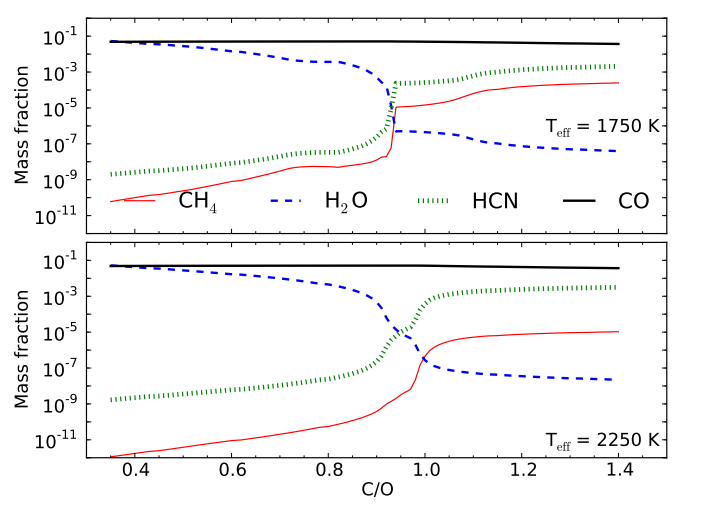
\includegraphics[width=0.7\textwidth]{CO_abundances}
%%\vspace{-0.5in}
%\caption{TBD}
%\label{fig:CO}
%\end{figure}

\begin{figure}[h!]
\centering
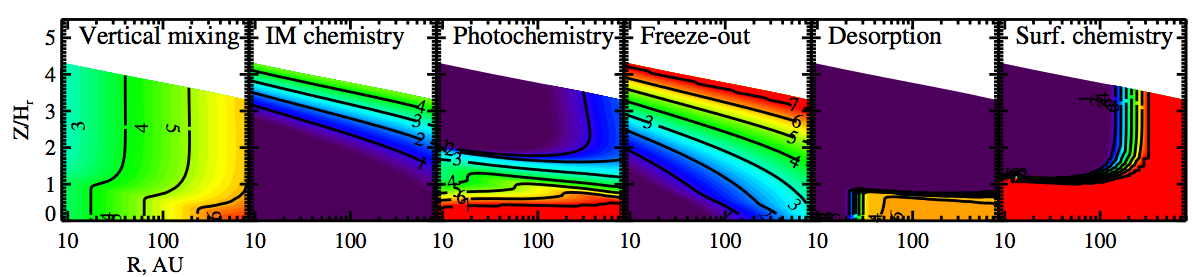
\includegraphics[width=\textwidth]{chemical_timescales}
%\vspace{-0.5in}
\caption{The distribution of characteristic chemical and dynamical timescales $\tau$ in disks as a function of semi-major axis and height. The numbered curves are $\log_{10} (\tau)$ in million years (from $[11]$).}
\label{fig:chemical}
\end{figure}

\begin{figure}[h!]
\centering
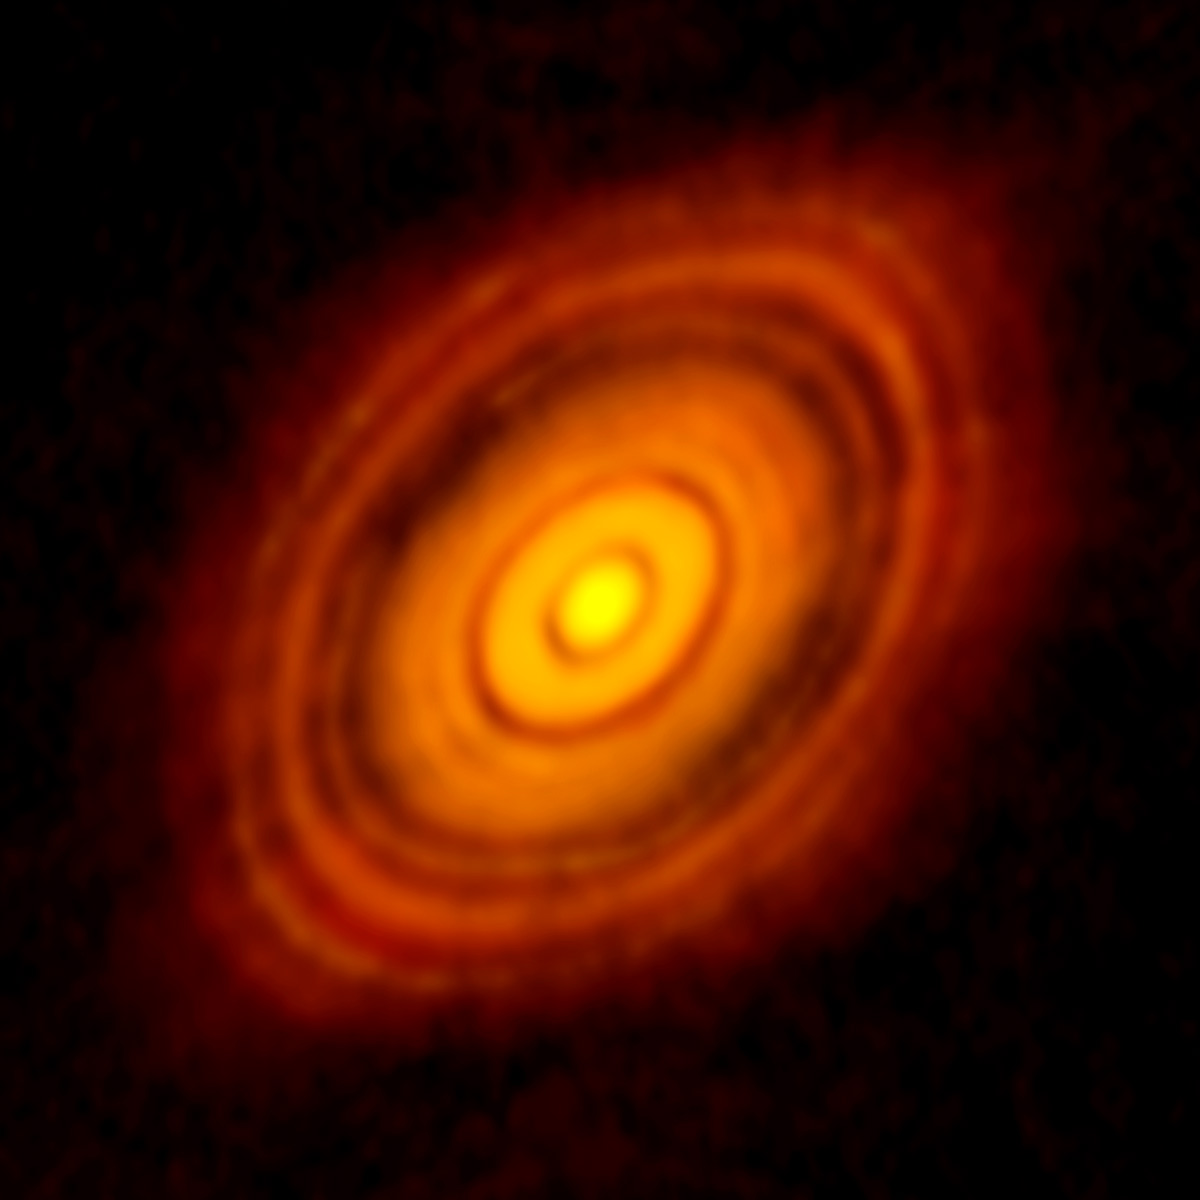
\includegraphics[width=0.4\textwidth]{HLTau_nrao}
%\vspace{-0.5in}
\caption{ALMA continuum image of the disk around HL Tau, which shows evidence of a gas gap in the disk, most likely created due to planetary migration (from $[8]$).}
\label{fig:HLTau}
\end{figure}

\begin{figure}[h!]
\centering
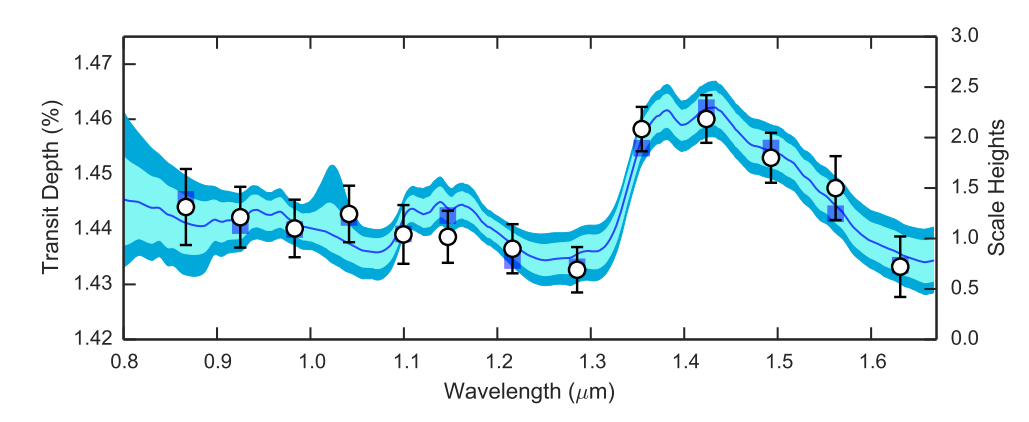
\includegraphics[width=0.9\textwidth]{water_spectrum}
%\vspace{-0.5in}
\caption{The transmission spectrum of exoplanet WASP-12b measured with the Hubble Space Telescope/Wide Field Camera 3. The white dots are the measured transit depths, the blue squares and dark blue line are the best fit model, while the shaded regions represent 1- and 2 $\sigma$ intervals in the retrieved spectrum. The increase in transit depth around $\sim$1.4 $\mu$m is evidence for a water feature in the atmosphere (from $[4]$).}
\label{fig:HLTau}
\end{figure}

%\if\bibinc n
%\bibliography{refs}
%\fi
\FloatBarrier
%\def\bibfont{\footnotesize}
%\setlength{\bibsep}{0.0pt}

\section*{References}
\footnotesize
%\begin{thebibliography} {9}
\noindent $[1]$ Batalha, N. M. 2014, Proceedings of the National Academy of Science, 111, 12647 \\
$[2]$ Lissauer J. J., Dawson R. I., Tremaine S., 2014, Nature, 513, 336 \\
$[3]$ Debes, J. H., Jang-Condell, H., Weinberger, A. J., Roberge, A., \& Schneider, G. 2013, ApJ, 771, 45 \\
$[4]$ Kreidberg, L., Line, M. R., Bean, J. L., et al. 2015, ArXiv e-prints, arXiv:1504.05586 \\
$[5]$ Piso, A.-M. A., \& Youdin, A. N. 2014, ApJ, 786, 21 \\
$[6]$ Piso, A.-M. A., Youdin, A. N., \& Murray-Clay, R. A. 2015, ApJ, 800, 82 \\
$[7]$ Piso, A.-M. A., �berg, K.I., Birnstiel, T, \& Murray-Clay, R.M., ApJ, resubmitted after referee report \\
$[8]$ ALMA Partnership et al., 2015, ApJ, 808, L3 \\
$[9]$ \"Oberg, K. I., Murray-Clay, R., \& Bergin, E. A. 2011, ApJ, 743, L16 \\
$[10]$ Ida, S., Lin, D. N. C., \& Nagasawa, M. 2013, ApJ, 775, 42 \\
$[11]$ Semenov, D., \& Wiebe, D. 2011, ApJS, 196, 25
%\end{thebibliography}

%\bibliographystyle{abbrv}
%\bibliography{refs}


%\if\bibinc y
%\begin{thebibliography}
%\end{thebibliography}
%\fi


\end{document}